\documentclass{article}


%INCLUDE
\usepackage[a4paper, left=20mm, right=20mm, top=20mm, bottom=20mm]{geometry}

\usepackage{amsmath, amsthm}
\usepackage[T1,T2A]{fontenc}
\usepackage[utf8]{inputenc}
%\usepackage[russian]{babel}
\usepackage{amssymb}
\usepackage{hyperref}
\usepackage{multirow}
\usepackage{stackengine}
\usepackage{algorithm}
\usepackage{algpseudocode}
\usepackage{lipsum}
\usepackage{authblk}
\usepackage{graphicx}
\usepackage{multicol}
\usepackage{pgfplots}
\usepackage{bm}
\usepackage{subcaption}
\usepackage{float} % for the H specifier
\usepackage{amsmath} % For \mathscr
\usepackage{mathrsfs} % For \mathscr
\usepackage{calrsfs} % For \mathcal
\usepackage{dutchcal} % For \mathdutchcal


%KHALED BEGIN

\usepackage{natbib}
\setcitestyle{authoryear,round,citesep={;},aysep={,},yysep={;}}

\renewcommand{\bibname}{References}
\renewcommand{\bibsection}{\subsubsection*{\bibname}}
\bibliographystyle{plainnat}

\usepackage[tableposition=top]{caption}
\usepackage{amsmath,amsthm,amssymb,mathtools,graphicx,enumitem,hyphenat,float, threeparttable}
\usepackage{mathabx, hyperref}
\hypersetup{ %
    pdfborder=0 0 0,
    pdfpagemode=UseNone,
    colorlinks=true,
    linkcolor=blue,
    citecolor=blue,
    filecolor=blue,
    urlcolor=blue,
    pdfview=FitH}
%KHALED END

%THEOREMS
\makeatletter
\def\th@plain{%
  \thm@notefont{}% same as heading font
}
\makeatother

\theoremstyle{plain}
\newtheorem{lemma}{Lemma}
\newtheorem{sublemma}{Sublemma}[lemma]


\theoremstyle{plain}
\newtheorem{assumption}{Assumption}

\theoremstyle{plain}
\newtheorem{statement}{Statement}

\theoremstyle{plain}
\newtheorem{corollary}{Corollary}

\theoremstyle{remark}
\newtheorem*{remark}{Remark}

\theoremstyle{plain}
\newtheorem{theorem}{Theorem}


%COMMANDS
\newcommand{\norm}[1]{\left\|#1\right\|}
\newcommand{\inner}[2]{\langle #1, #2\rangle}
\newcommand{\summ}[3]{\sum^{ #2 }_{ #1 } #3}
\newcommand{\fsumm}[3]{\frac{1}{M}\sum^{ #2 }_{ #1 } #3}
\newcommand{\coef}[1]{\biggr[ #1 \biggr]}
\newcommand{\E}{\mathbb{E}}
\newcommand{\mc}{\mathcal}


\newcommand{\greencheck}{{\color{green}\checkmark}}
\newcommand{\redcross}{{\color{red}\textbf{\texttimes}}}
\newcommand{\smallfont}[1]{{\small #1}}
\begin{document}

%TITLE
%TITLE

\title{\fontsize{12}{14}\selectfont \textbf{Enhancing the convergence estimate of Local SGD for target functions of a special type/ Local SGD converges faster for quadratic-like functions independent of the Hessian}}

\author[1]{\fontsize{11}{14} \textbf{Andrei Sadchikov}}
\author[1, 2]{\fontsize{11}{14} \textbf{Aleksandr Beznosikov}}
\author[1, 3]{\fontsize{11}{14} \textbf{Alexander Gasnikov}}
\affil[1]{MIPT}
\affil[2]{University Two}
\affil[3]{University Three}

\date{}

%BEGIN
\maketitle

%ABSTRACT
\begin{abstract}
One of the challenges of Federated learning is finding the right balance in communication frequency: too infrequent communications lead to worse convergence, while too frequent ones require significant overhead (time for data transmission and network load). 
\cite{Woodworth} proved that for the case where the objective function is quadratic, the communication frequency does not affect the upper bound on the convergence rate.
In this work, we focus on generalizing these results, providing an analysis in the case where the objective function is the sum of a quadratic function and an arbitrary remainder.
\end{abstract}

%MAIN BODY
%INTRODUCTION
\section{Introduction}

Before we talk about our contributions, let's quickly explain what Federated Learning is and what problem it's solving.

\subsection{General words}

In the ever-evolving landscape of machine learning, we've witnessed the emergence of enormous models like Gemini, boasting trillions of parameters that push the boundaries of computational capacity. Given the impracticality of training such models on a single device, modern machine learning has embraced Federated Learning, a concept initially introduced by \cite{McMahan}. This approach involves distributing data across multiple devices, each conducting local computations, and subsequently communicating to collectively achieve the final result.

\vspace{10pt}

However, the challenge of communication frequency remains unresolved in Federated Learning. Insufficient communication may lead to divergence, while overly frequent communication poses its own set of issues. Imagine tackling an optimization problem in a space with a dimension around $10^9$, which occurs often in practice \citep{shahid2021communication}. Each time we compute a gradient locally, it ends up being gigabytes in size, which makes sending it over for transmission quite a challenge. Thus, striking the delicate balance in communication frequency becomes the key to success in Federated Learning.

\vspace{10pt}

To address this challenge, scientific community has developed sophisticated federated learning frameworks capable of performing well even with infrequent communication. Among the most notable are SCAFFOLD \citep{Scaffold} and FedAC \citep{FedAC}. These algorithms are widely utilized in practice since they save a lot of time on communication. They also show efficiency when data distribution varies among computational devices \citep{Hospitals}. Unfortunately, due to their complexity, implementation and convergence analysis of such algorithms can be challenging.

\vspace{10pt}

On the other hand, the simplest and most classical algorithm that also utilizes the idea of rare communications, named Local SGD (also known as FedAvg or Parallel SGD), has been proven to be as efficient as these intricate algorithms when data distribution is similar \citep{KEK LOL}. 
The core concept of Local SGD can be described as follows: each participating device conducts few steps of SGD locally and then devices communicate with each other averaging their models' weights (see~\ref{subsec:problem_formulation} for more details)

\vspace{10pt}

Even though idea is not new, and it was introduced more that two decades ago by \cite{Mangasarian}, Local SGD is now again in the center of attention.
It's pluses made the algorithm attractive for both practitioners, due to the communication complexity combined with the ease of implementation, and theoreticians, due to the simplicity of it's analysis. 

\vspace{10pt}

In environments where the distribution of data remains similar, such as when computations are distributed within a computational cluster or among processor cores within a single device, Local SGD finds extensive application. This classical algorithm remains actively utilized in modern machine learning applications such as Natural Language Processing (NLP) and computer vision. Recent studies \citep{LocalSGD_LLM, LocalSGD_CV} have underscored its efficiency and effectiveness in identical distribution situations. With its straightforward approach and strong performance, Local SGD continues to play pivotal role in training large models. In this paper, we concentrate on analyzing convergence rates for Local SGD.

\vspace{10pt}

\subsection{Problem formulation} \label{subsec:problem_formulation}

Now, let us formally introduce the task we are solving. Consider a scenario where \( M \) devices \( 1, 2, \ldots, m \), collectively solving optimization problem, that is finding:

\[ x_* := \arg\min_{x \in \mathbb{R}^d} F(x) \]

Here, \( F(x) \) is defined as the expected value over a distribution \( \mathcal{D} \):

\[ F(x) := \mathbb{E}_{z \sim \mathcal{D}} [F(x, z)] \]

%where \( z \) is sampled from the distribution \( \mathcal{D} \).

Our focus lies on a first-order stochastic oracle, where we have access to the stochastic estimate of \( \nabla F \) on each node. We denote this estimate as \( \nabla F(x, z) \), with \( z \) representing a sample from \( \mathcal{D} \).

\vspace{10pt}

This formulation captures a wide range of practical problems, such as Empirical Risk Minimization \citep{Vapnik}. In our case \( F \) denotes the empirical risk (i.e., the average of losses across some data samples) and \( z \) denotes the indices of data samples.

\vspace{10pt}

Here it is important to underline the method by which we measure communication complexity for Federated Learning methods. Unlike classical optimization, where complexity was considered as the number of times the oracle is called, i.e., computing local gradients $\nabla F(x^m, z^m)$, we also care about communication complexity. Generally, we define it as the quantity of information we transmit, or the number of communications in our case.
So, in this work, we will emphasize reducing the number of communication rounds $R$ or increasing the number of SGD steps between communications, denoted as $H$, while keeping the total number of SGD steps $T$ unchanged.

\vspace{10pt}

Now we are ready to get familiar with the formal definition of Local SGD.

\begin{algorithm} \label{alg:localsgd}
    \caption{Local SGD}
    \begin{algorithmic}[1]
        \State \textbf{Input:} 
        Initial vector $x_0 = x^m_0$ for all $m \in \{1, \ldots, M\}$; 
        stepsize $\gamma \geq 0$
        \For{$t = 1, \ldots, T = R\cdot H$}
            \For{$m = 1, \ldots, M$ in parallel}
                \State Sample $z^m_t \sim \mathcal{D}$.
                \State Evaluate stochastic gradient $\mc{g}_t^m = \nabla F(x_t^m, z^m_t)$.
            \EndFor
            \If{$t+1 \mod H = 0$}
                \State $x^m_{t+1} = \frac{1}{M} \sum^M_{j = 1} (x^j_t - \gamma \mc{g}^j_t) $
            \Else
                \State $x^m_{t+1} = x_t^m - \gamma \mc{g}_t^m$ \label{eq:upd_eq}
            \EndIf
        \EndFor
    \end{algorithmic}
\end{algorithm}

\vspace{10pt}

\subsection{Related work}

In both scenarios of identical and heterogeneous settings, extensive research has been conducted across various contexts. \cite{Li} and \cite{haddapour} analyzed the non-convex setting under bounded gradient norms. As expected, the further we deviate from the identical and strongly convex settings, the poorer the results become. However, in this work, we will focus solely on convex and strongly convex cases.

\vspace{10pt}

The theoretical aspect of the convex case has been extensively studied. Among the most remarkable works, we can mention \cite{Stich}, who conducted analysis under the assumption of bounded gradient norms. Subsequently, a considerable amount of research was conducted on integrating Local SGD with various Federated Learning techniques, such as momentum, quantization, and restarting \citep{fedpaq, spider, restarts}.

\vspace{10pt}

Notably, \cite{Khaled} and \cite{Woodworth} provided the best known estimate without any restrictions of the Hessian. In our study, we extend these findings, particularly in cases where the objective function $F$ exhibits proximity to a quadratic form. Importantly, our approach does not assume Hessian Lipschitzness as other works \cite{FedAC}, thus representing a generalization of previous research efforts.

\vspace{10pt}

It's worth noting that the majority of existing research, with the exception of \cite{Spiridonoff}, operates under the assumption that the variance of stochastic gradients is uniformly bounded. This assumption posits the existence of a constant $\sigma$ such that $\norm{\nabla F(x, z) - \nabla F(x)}^2 \leq \sigma^2$. However, this assumption is often unrealistic in real-world scenarios. For example, it is violated in the case of Coordinate SGD \citep{coordinateSGD}, where only a subset of partial derivatives is computed instead of the full gradient. Therefore, one of our objectives was to analyze Local SGD for quadratic-like functions under assumption~\ref{ass:ass_2}, which seems to be very general and hold almost always.

\begin{table}[H]

\caption{Summary of similar works}

\renewcommand{\arraystretch}{2} % Increase the height of each row
\begin{adjustwidth}{-5cm}{-5cm} % Adjust the margins by -1cm on each side
\centering
\footnotesize

\begin{threeparttable}
\begin{tabular}{|p{2cm}|p{1.7cm}|p{1.7cm}|p{1.5cm}|p{1.5cm}|p{6cm}|}
\hline
\textbf{Reference} &
\textbf{Not-Lipschitz Hessian} &
\textbf{Unbounded Gradient} &
\textbf{Noise model} &
\textbf{Convexity} & 
\textbf{Convergence rate, $\E[F(.)] - F(x_=) \leq$} \\

% \hline

% %_____________________%
% \multirow{2}{=}{Vanila SGD} &
% \multirow{2}{=}{\greencheck} &
% \multirow{2}{=}{\greencheck} &
% \multirow{2}{=}{Uniform} 
% & 
% $\mu=0$ & $O(exp.decay + \frac{A}{B})$ \\
% & & & & 
% $\mu > 0$ & $O(exp.decay + \frac{A}{B})$ \\
% %_____________________%

\hline

%_____________________%
\multirow{2}{=}{\cite{Stich}} &
\multirow{2}{=}{\redcross (?)} &
\multirow{2}{=}{\redcross} &
\multirow{2}{=}{Uniform} 
& 
$\mu=0$ & - \\
& & & & 
$\mu > 0$ & $\O \left(
  			\frac{D^2}{R^3} + \frac{\sigma^2}{\mu M T} + 
  			\frac{\kappa G^2}{\mu R^2} \right)$ \tnote{{\color{blue}(G-note)}} \\
%_____________________%

\hline

%_____________________%
\multirow{2}{=}{\cite{FedAC}} &
\multirow{2}{=}{\redcross} &
\multirow{2}{=}{\greencheck} &
\multirow{2}{=}{Uniform} 
& 
$\mu=0$ & $\tilde{\O} \left( 
            \frac{LD^2}{T} + \frac{\sigma D}{\sqrt{MT}} + \frac{Q^{\frac{1}{3}} \sigma^{\frac{2}{3}} D^{\frac{5}{3}}}{T^{\frac{1}{3}} R^{\frac{1}{3}}}
        \right)$ \tnote{{\color{blue}(Q-note)}} \\
& & & & 
$\mu > 0$ & $\tilde{\O} \left(\text{exp. decay} + \frac{\sigma^2}{\mu M T} + \frac{Q^2                     \sigma^4}{\mu^5 T^2 R^2}   \right)$ \\
%_____________________%

\hline

%_____________________%
\multirow{2}{=}{\cite{Spiridonoff}} &
\multirow{2}{=}{\greencheck} &
\multirow{2}{=}{\greencheck} &
\multirow{2}{=}{Uniform with strong growth \tnote{{\color{blue}($\rho$-note)}}} 
& 
$\mu=0$ & - \\
& & & & 
$\mu > 0$ & $\O \left( 
  			\frac{(1 + \rho \kappa^2\ln(TR^{-2})) D^2}{\kappa^{-2}T^2} + 
  			\frac{\kappa \sigma^2}{\mu M T} + \frac{\kappa^2 \sigma^2}{\mu T R}\right) \\
%_____________________%

\hline

%_____________________%
\multirow{2}{=}{\cite{Khaled}} &
\multirow{2}{=}{\greencheck} &
\multirow{2}{=}{\greencheck} &
\multirow{2}{=}{Uniform} 
& 
$\mu=0$ & ${\O} \left(
          \frac{D^2}{\sqrt{MT}} + \frac{\sigma^2}{L\sqrt{MT}} + \frac{\sigma^2 M}{LR}
          \right)$ \tnote{{\color{blue}(improve-lr)}} \\ 
& & & & 
$\mu > 0$ & $\tilde{\O} \left( 
  			\frac{L D^2 }{T^2} + 
  			\frac{L \sigma^2}{\mu^2 M T} + \frac{L^2 \sigma^2}{\mu^3 T R} \right)$ \\
%_____________________%

\hline

%_____________________%
\multirow{4}{=}{\textbf{This work}} &
\multirow{2}{=}{\greencheck} &
\multirow{2}{=}{\greencheck} &
\multirow{2}{=}{Uniform} 
& 
$\mu=0$ & ${\O} \left(
          \frac{D^2}{\sqrt{MT}} + \frac{\sigma^2}{L\sqrt{MT}} + \frac{
          \bm{\varepsilon} \sigma^2 M}{LR} \right)$ 
          \tnote{{\color{blue}($\varepsilon$-note)}}
          \\
          
& & & & 
$\mu > 0$ & $\tilde{\O} \left( 
  			\frac{L D^2 }{T^2} + 
  			\frac{L \sigma^2}{\mu^2 M T} + \frac{
     \bm{\varepsilon} L^2 \sigma^2}{\mu^3 T R} \right)$ 
     \\
%_____________________%

\cline{2-6}

%_____________________%
\multirow{4}{=}{} &
\multirow{2}{=}{\greencheck} &
\multirow{2}{=}{\greencheck} &
\multirow{2}{=}{Uniform with strong growth} 
& 
$\mu=0$ & - \\
& & & & 
$\mu > 0$ & - \\
%_____________________%

\hline

\end{tabular}
\begin{tablenotes}
\begin{itemize}
    \item General notation: 
    $\O$ omits constant factors;
    $\tilde{\O}$ omits polylogarithmic and constant factors.
    $D = \norm{x_0-x_*}$ - initial distance from minimum;
    $\sigma$ - variance of stochastic gradient, see ass.~\ref{ass:ass_2}; 
    $\mu$ is a strong convexity constant 
    and $L$ is a Lipshitz gradient constant, see ass.~\ref{ass:ass_1};
    $M$ - number of workers;
    $R$ - number of communication rounds;
    $T$ - total number of iterations. For more detailed explanation see table~\ref{tab:notation}
    
    \item \tnote{{\color{blue}($\rho$-note)}} $\rho$ came from ass.~\ref{ass:ass_2}

    \item \tnote{{\color{blue}(improve-lr)}} Шаг следует выбрать поинтереснее
    
    \item \tnote{{\color{blue}($\varepsilon$-note)}} $\varepsilon$ shows how far function is from quadratic; 
    for all functions $\varepsilon \leq 1$ and for quadratic functions $\varepsilon = 0$. For more details see st.~\ref{st:st_1} and section~\ref{sec:discussion}
\end{itemize}
\end{tablenotes}
\end{threeparttable}

\end{adjustwidth} % End of adjustwidth environment

\label{tab:different_row_counts}

\end{table}


As evident from this table, our work achieves a clear improvement in the estimates obtained by \cite{Khaled}.

% The rest of this paper is organized as follows. In the following section we outline the related
% literature and compare existing results. In subsection~\ref{subsec:settings} we define the main problem and state our assumptions.
% We present our theoretical findings in subsection~\ref{subsec:contributions}  followed by numerical experiments in section~\ref{sec:experiments} and
% proofs in section~\ref{sec:proofs}.


\subsection{Specifics of the quadratic case}

\cite{earlyquadratics} were the first to notice that in the scenario where the objective function is quadratic, the convergence rate of Local SGD remains independent of communication frequency. Later, \cite{Woodworth} provided a proof of this. This important observation aligns with the lower bounds established for Local SGD, indicating that for purely quadratic functions, further enhancement of the convergence rate is unattainable.

\vspace{10pt}

Subsequent works focused on the generalization of this. Unsurprisingly, the most promising outcomes in the identical convex case, where the function is not quadratic, were previously achieved under the assumption of a Lipschitz Hessian \citep{FedAC, Spiridonoff}, because this assumption in some way demonstrates the "quadraticity" of a function.

\vspace{10pt}

However, a gap still exists between the general case, as analyzed by \cite{Khaled}, and the challenging assumption of a Lipschitz Hessian. This assumption appears to be invalid for neural networks with ReLU activation functions. Therefore, our primary objective is to offer an analysis that bridges this gap. To achieve this, we introduce the concept of "\textbf{quadraticity}", i.e. $\varepsilon$ (\ref{st:st_1}), which provides insight into the proximity of a function to a quadratic form without imposing additional assumptions and conduct our analysis with respect to the "quadraticity" of the objective function.


%SETTINGS AND CONTRIBUTIONS
\section{Contributions} 
\subsection{Contributions} \label{subsec:contributions}

In this work, we mainly focus on the improvement in the last term of both convergence rates provided by Khaled et al. in prospect of statement~\ref{st:st_1}.

%THEOREM 1
\begin{theorem} \label{th:th_1}
    Under assumptions~\ref{ass:ass_1} and~\ref{ass:ass_2}, decomposing $F$ as announced in~\ref{st:st_1} and considering $\mu > 0$ and $\gamma \leq \frac{1}{6 L}$ gives:
    \begin{align}
        \E \norm{\bar{x}_T - x_*}^2
        \leq
        (1 - \gamma \mu)^T \norm{x_0 - x_*}^2 
        + \frac{\gamma \sigma^2}{\mu M} 
        + \frac{2 \varepsilon \gamma^2 \sigma^2 L (H-1)}{\mu}
    \end{align}
\end{theorem}

\begin{corollary} \label{}
    As it was previously shown in \cite{Woodworth}, an important special case is is achieved when epsilon is equal to zero. Than from the Theorem~\ref{th:th_1} it follows that:
    \begin{align}
        \E[\norm{\bar{x}_T - x_*}^2]
        \leq
        (1 - \gamma \mu)^T \norm{x_0 - x_*}^2 
        + \frac{\gamma \sigma^2}{\mu M}
    \end{align}
\end{corollary}

Thus, if $F$ is a quadratic function, the upper bound on the rate of convergence is independent of the communication frequency.

\begin{corollary} \label{}
    Considering $\gamma$ as a function of $t$ and choosing $\gamma_t$ as in Theorem 2 from \cite{Woodworth}, we obtain:
    \begin{align}
        \E[F(\bar{x}_t) - F(x_*)]
        \leq
        c \cdot \left(
        \text{exp} \left(-\frac{\mu T}{4 L}\right) +
        \frac{\sigma^2}{\mu MT} + \frac{\varepsilon \sigma^2}{\mu^2 TR}
        \right)
    \end{align}
    Where $c \in \mathbb{R}$ is some universal constant.
\end{corollary}



%THEOREM 2
\begin{theorem} \label{th:th_2}
    Under assumptions~\ref{ass:ass_1} and~\ref{ass:ass_2}, decomposing $F$ as announced in~\ref{st:st_1} and considering $\mu = 0$ and $\gamma \leq \frac{1}{6 L}$ we have:
    \begin{align}
        \E[F(\hat{x}_T)] - F(x_*) \leq
        \frac{2}{\gamma T} + \frac{2 \gamma \sigma^2}{M} + 12 \varepsilon \gamma^2 L \sigma^2 (H-1)
    \end{align}
    Where $\hat{x}_T = \frac{1}{T} \summ{t=1}{T} \bar{x}_t$
\end{theorem}

\begin{corollary} \label{}
    Choosing $\gamma = \frac{\sqrt{M}}{6 L\sqrt{T}}$ and assuming $M \leq T$ as in \cite{Khaled} yields:
    \begin{align}
        \E[F(\hat{x}_T)] - F(x_*)
        \leq
          \frac{12 \norm{x_0-x_*}^2}{\sqrt{MT}} + \frac{\sigma^2}{3 L\sqrt{MT}} + \frac{
          \varepsilon \sigma^2 M}{3LR}
    \end{align}
\end{corollary}


\section{Settings} 

%Convexity and nabla-Lipschitzness
\begin{assumption} \label{ass:ass_1}
    Assume that $F$ is $\mu$-convex and $L$-smooth. That is, $\forall x, y \in \mathbb{R}^d$,
    \[
    \frac{\mu}{2} \norm{x - y}^2 \leq F(y) - F(x) - \inner{\nabla F(x)}{y-x} \leq \frac{L}{2} \norm {x-y}^2
    \]
\end{assumption}

\begin{corollary} \label{cor:nesterov}
Under assumption~\ref{ass:ass_1}
    \[
    \frac{1}{2L} \norm{\nabla F(x) - \nabla F(y)}^2 \leq F(y) - F(x) - \inner{\nabla F(x)}{y-x}
    \]
\end{corollary}
\proof{
    This is Theorem 2.1.5 in \cite{Nesterov}
}


%Bounded stochastic gradient variance
\begin{assumption} \label{ass:ass_2}
    Exist such constants $\sigma$ and $\rho$ that:
    \[\E_{z \sim \mathcal{D}} \norm {\nabla F(x, z) - \nabla F(x)}^2 \leq \sigma^2
    + \rho \norm{\nabla F(x)}^2 \]
\end{assumption}

\begin{assumption} \label{ass:ass_3}
    The stochastic gradient is an unbiased estimate of its expectation:
    \[ \E_{z \sim \mathcal{D}}[\nabla(F(x, z)] = F(x)\]
\end{assumption}

%F=Q+R decomposition
\begin{statement}[\varepsilon - decomposition] \label{st:st_1}
    Objective function can be decomposed as $F = Q + R$, where $Q$ is a quadratic function that is $\mu_Q$-convex and $L_Q$-smooth, and $R$ is $\mu_R$-convex and $L_R$-smooth. Than we denote parameter
    \(\varepsilon := \frac{L_R}{L}\)
    which gives us an idea of how far $F$ is from a quadratic function.
\end{statement}

Note that such decomposition always takes place because we can take $Q = 0$ and $R = F$.

We will denote the sum of $\mu_Q$ and $\mu_R$ as $\lambda$, and $\frac{L}{\lambda}$ as $\kappa$. 

\begin{corollary} \label{cor:linearity}
    In the prospect of Statement~\ref{st:st_1}, following takes place: $\,$
    \begin{enumerate}
    \item[a)] $\nabla Q$ is a linear function
    \item[b)] \(\varepsilon \leq 1\)

    \item[c)] \(\lambda \leq \mu\)
\end{enumerate}
\end{corollary}

%DISCUSSION
\section{Discussion}
Things get more interesting in perspective of expressing $\E[\norm{\bar{x}_{t+1} - x_*}^2]$ through $\E[\norm{\bar{x}_{t} - x_*}^2]$ instead of solving recurrent relation and analyzing $\E[\norm{\bar{x}_T - x_*}^2]$. 

%We'll go deeper into the strongly convex case because it's more intuitive.

As can be observed from~\ref{lem:main}:
\begin{align}
     \E \norm{\bar{x}_{t+1}-x_*}^2
    &\leq
    (1 - \gamma \mu) \E \norm{\bar{x}_t - x_*}^2 
    + \frac{\gamma^2 \sigma^2}{M}
    + 10 \varepsilon \gamma L (H-1) \gamma^2 \sigma^2 \label{eq:recurrent}
\end{align}

Considering $\varepsilon$ as a function of $x$, we can say that for the functions with Lipschitz Hessian we know that the decay rate of $\varepsilon$ is fast. Following graphs illustrate decay rate of $\varepsilon$ for some functions:

\begin{figure}[H] \label{graph:eps_graphs}
\centering
\begin{subfigure}{0.3\textwidth}
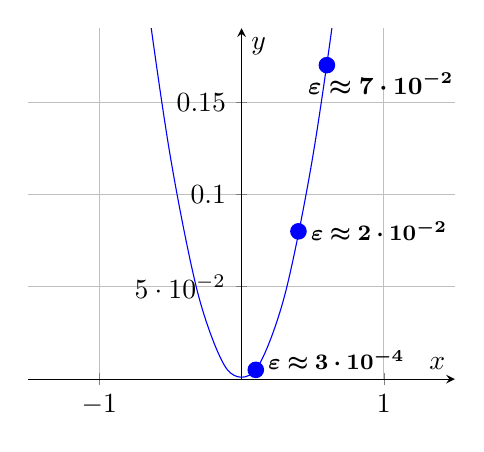
\begin{tikzpicture}
\begin{axis}[
    width=7cm,
    xlabel={$x$},
    ylabel={$y$},
    xmin=-1.5, xmax=1.5,
    ymin=0, ymax=0.19, % Adjust y-axis limits
    axis lines=center,
    grid=both,
    domain=-10:10,
    samples=100,
    % restrict y to domain=-2.5:2.5 % Restrict y-axis domain
]

\addplot[blue, smooth] {ln(cosh(x))};

\coordinate (A1) at (axis cs:0.6,0.17);
\coordinate (B1) at (axis cs:0.4,0.16);

\fill[blue, thick] (A1) circle (3pt);
\node[right] at (B1) {\small $\bm{\varepsilon \approx 7 \cdot 10^{-2}}$};

%\draw[dashed] (A1) -- (B1);
 %----------------------------------------%
\coordinate (A2) at (axis cs:0.4,0.08);
\coordinate (B2) at (axis cs:0.42,0.08);

\fill[blue, thick] (A2) circle (3pt);
\node[right] at (B2) {\footnotesize $\bm{\varepsilon \approx 2 \cdot 10^{-2}}$};

%\draw[dashed] (A2) -- (B2);
 %----------------------------------------%
% \coordinate (A3) at (axis cs:0.2,0.02);
% \coordinate (B3) at (axis cs:0.35,0.03);

% \fill[blue, thick] (A3) circle (3pt);
% \node[right] at (B3) {\footnotesize $\bm{\varepsilon \approx 2 \cdot 10^{-3}}$};

% \draw[dashed] (A3) -- (B3);
%----------------------------------------%
\coordinate (A4) at (axis cs:0.1,0.005);
\coordinate (B4) at (axis cs:0.12,0.01);

\fill[blue, thick] (A4) circle (3pt);
\node[right] at (B4) {\footnotesize $\bm{\varepsilon \approx 3 \cdot 10^{-4}}$};

%\draw[dashed] (A4) -- (B4);

\end{axis}
\end{tikzpicture}
\caption{LogCoshLoss: $y = \ln(\cosh(x))$ }
\end{subfigure}
\hfill
\begin{subfigure}{0.3\textwidth}
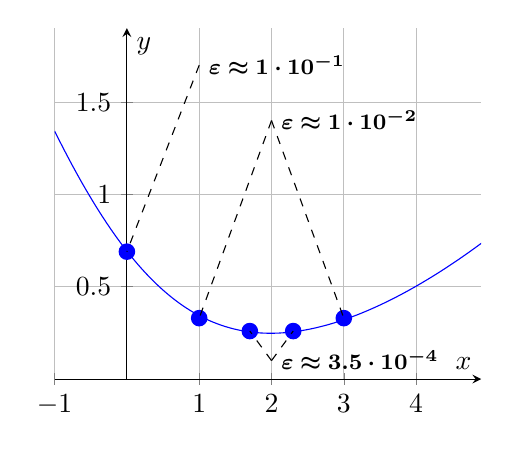
\begin{tikzpicture}
\begin{axis}[
    width=7cm,
    xlabel={$x$},
    ylabel={$y$},
    xmin=-1, xmax=4.9,
    ymin=-0, ymax=1.9,
    axis lines=center,
    grid=both,
    samples=100,
]
\addplot[blue, domain=-1:5] {-ln(1/(1 + exp(-x))) + x^2/33};

\coordinate (A1) at (axis cs:1, 0.33);
\coordinate (B1) at (axis cs:2, 1.4);
\coordinate (C1) at (axis cs:3,0.33);

\fill[blue, thick] (A1) circle (3pt);
\fill[blue, thick] (C1) circle (3pt);
\node[right] at (B1) {\footnotesize $\bm{\varepsilon \approx 1 \cdot 10^{-2}}$};

\draw[dashed] (B1) -- (A1);
\draw[dashed] (B1) -- (C1);
 %----------------------------------------%
\coordinate (A2) at (axis cs:1.7, 0.26);
\coordinate (B2) at (axis cs:2, 0.1);
\coordinate (C2) at (axis cs:2.3,  0.26);

\fill[blue, thick] (A2) circle (3pt);
\fill[blue, thick] (C2) circle (3pt);
\node[right] at (B2) {\footnotesize $ \bm{\varepsilon \approx 3.5 \cdot 10^{-4}}$};

\draw[dashed] (B2) -- (A2);
\draw[dashed] (B2) -- (C2);
 %----------------------------------------%
 \coordinate (A2) at (axis cs:0, 0.69);
\coordinate (B2) at (axis cs:1, 1.7);

\fill[blue, thick] (A2) circle (3pt);
\node[right] at (B2) {\footnotesize $\bm{\varepsilon \approx 1 \cdot 10^{-1}}$};

\draw[dashed] (B2) -- (A2);
 %----------------------------------------%
\end{axis}
\end{tikzpicture}
\caption{LogLoss with $l_2$ reg.  ~\eqref{eq:logloss}}
\end{subfigure}
\hfill
\begin{subfigure}{0.3\textwidth}
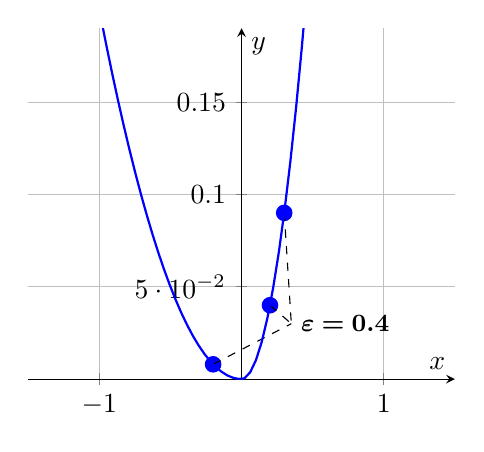
\begin{tikzpicture}[
  declare function={
    func(\x)= (\x < 0) * (x*x/5)   +
              (\x >= 0) * (x*x)
   ;
  }
]
\begin{axis}[
    width=7cm,
    xlabel={$x$},
    ylabel={$y$},
    xmin=-1.5, xmax=1.5,
    ymin=0, ymax=0.19, % Adjust y-axis limits
    axis lines=center,
    grid=both,
    domain=-2:2,
    samples=100,
    % restrict y to domain=-2.5:2.5 % Restrict y-axis domain
]

\coordinate (A1) at (axis cs:-0.2,0.008);
\coordinate (A2) at (axis cs:0.2,0.04);
\coordinate (A3) at (axis cs:0.3,0.09);

\coordinate (B1) at (axis cs:0.35,0.03);

\fill[blue, thick] (A1) circle (3pt);
\fill[blue, thick] (A2) circle (3pt);
\fill[blue, thick] (A3) circle (3pt);


\node[right] at (B1) {\small $\bm{\varepsilon = 0.4}$};

\draw[dashed] (A1) -- (B1);
\draw[dashed] (A2) -- (B1);
\draw[dashed] (A3) -- (B1);

\addplot [blue,thick] {func(x)};
\end{axis}
\end{tikzpicture}
\caption{Lower-bound function $\mathcal{F} $ ~\eqref{eq:piecewise}}
\end{subfigure}


\caption{Decay of $\varepsilon$ when getting closer to minima}
\end{figure}
\\

In point (b) by LogLoss we mean 
\begin{equation} \label{eq:logloss}
    y = -\ln\left(\frac{1}{1 + e^{-x}} \right) + 0.03 {x^2}
\end{equation}

And in point (c) we analyze well-known function that yields lower bound estimates for Local SGD \citep{LowerBound}.
\begin{equation} \label{eq:piecewise}
    \mathcal{F}(x) = \begin{cases} 
      x^2 / 5 & \text{if } x < 0 \\
      x^2 & \text{if } x \geq 0 \\
   \end{cases}
\end{equation}

Here we can notice that for functions (a) and (b) $\varepsilon$ decreases rapidly (because they satisfy Lipschitz Hessian assumption), and for function (c) it remains constant. This may be considered as some additional insight into why 
$\mathcal{F}$ yields lower bound for Local SGD.

From this example we can observe that equation~\ref{eq:recurrent} provides valuable insights into convergence rate for different types of functions. However, abandoning the assumption of a Lipschitz Hessian means that we cannot estimate the decay rate of epsilon. Therefore conducting a meaningful asymptotic analysis while maintaining generality seems impossible.

Thus our aim is to present our findings within a broader scope, elucidating the physical interpretation of the convergence rate.


%REFERENCES
\bibliographystyle{plain}
\bibliography{bibliography.bib}

%SUPPLEMENTARY MATERIAL
%CONTENTS
\tableofcontents
\newpage

%PROOFS
\section{Proofs} \label{sec:proofs}

\subsection{Notation}
$ $\par
Let us introduce useful contractions:
\begin{align}
    &\mc{g}^m_t := \nabla F(x^m_t, z^m_t) \\
    &\mc{r}^m_t := \nabla R(x^m_t, z^m_t) \\
    &\mc{q}^m_t := \nabla Q(x^m_t, z^m_t) \\
    &g^m_t := \nabla F(x^m_t) \\
    &r^m_t := \nabla R(x^m_t) \\
    &q^m_t := \nabla Q(x^m_t) \\
\end{align}

Also for average values:
\begin{align}
    &\bar{r}_t := \fsumm {m=1}{M}{\nabla R(x^m_t)} \\
    &\bar{R}_t := \fsumm {m=1}{M}{R(x^m_t)} \\
    &\bar{q}_t := \fsumm {m=1}{M}{\nabla Q(x^m_t)} \overset{\text{~\ref{cor:linearity}}}{=}  \nabla Q(\bar{x}_t)
\end{align}

And for values of $Q$ and $R$ at $x_*$:
\begin{align}
    &r_* := \nabla R(x_*)
    &R_* := R(x_*) \\
    &q_* := \nabla Q(x_*)
    &Q_* := Q(x_*)
\end{align}

\subsection{Technical lemmas}

Before demonstrating the claimed facts, let's first establish some technical results.
In this section we will follow the path of proving Lemma 3.1 from \cite{Stich}.

\begin{lemma} \label{lem:lem_1}
    \begin{align*}
        \norm{\bar{x}_t - x_* - \gamma \bar{g}_t}^2
        &= \norm{\bar{x}_t - x_*}^2 
        + \gamma^2 \norm{\bar{q}_t 
        + \bar{r}_t - q_* - r_*}^2 
        - 2 \gamma \inner{\bar{x}_t - x_*}{\bar{q}_t}
        - 2 \gamma \inner{\bar{x}_t - x_*}{\bar{r}_t} 
    \end{align*}
\begin{proof}
    \begin{align*}
        \norm{\bar{x}_t - x_* - \gamma \bar{g}_t}^2
        &= 
        \norm{\bar{x}_t - x_*}^2 
        + \gamma^2 \norm{\bar{g}_t}^2 
        - 2 \gamma \inner{\bar{x}_t - x_*}{\bar{g}_t} \\
        &= 
        \norm{\bar{x}_t - x_*}^2 
        + \gamma^2 \norm{\bar{g}_t}^2 
        - \frac{2\gamma}{M} \summ {m=1}{M}{ \inner{\bar{x}_t - x_*}{\nabla F(x^m_t)} } \\
        &= 
        \norm{\bar{x}_t - x_*}^2 
        + \gamma^2 \norm{\fsumm {m=1}{M}{\nabla F(x^m_t)}}^2 
        - \frac{2\gamma}{M} \summ {m=1}{M}{ \inner{\bar{x}_t - x_*}{\nabla F(x^m_t)} } \\
        &= 
            \notag
        \norm{\bar{x}_t - x_*}^2 
        + \gamma^2 \norm{\fsumm {m=1}{M}{\nabla F(x^m_t)} - \nabla F(x_*)}^2 
        - \frac{2\gamma}{M} \summ {m=1}{M}{ \inner{\bar{x}_t - x_*}{\nabla F(x^m_t)} } \\
        &= 
            \notag
        \norm{\bar{x}_t - x_*}^2 
        + \gamma^2 \norm{\fsumm {m=1}{M}{\nabla Q(x^m_t) + \nabla R(x^m_t) - \nabla Q(x_*) - \nabla R(x_*)}}^2  \\
        &- \frac{2\gamma}{M} \summ {m=1}{M}{ \inner{\bar{x}_t - x_*}{\nabla Q(x^m_t)} }
        - \frac{2\gamma}{M} \summ {m=1}{M}{ \inner{\bar{x}_t - x_*}{\nabla R(x^m_t)} }  \\
        &= 
        \norm{\bar{x}_t - x_*}^2 
        + \gamma^2 \norm{\bar{q}_t 
        + \bar{r}_t - q_* - r_*}^2  
        - \frac{2\gamma}{M} \summ {m=1}{M}{ \inner{\bar{x}_t - x_*}{q^m_t} }
        - \frac{2\gamma}{M} \summ {m=1}{M} { \inner{\bar{x}_t - x_*}{r^m_t} } \\
        &= 
        \norm{\bar{x}_t - x_*}^2 
        + \gamma^2 \norm{\bar{q}_t 
        + \bar{r}_t - q_* - r_*}^2 
        - 2 \gamma \inner{\bar{x}_t - x_*}{\bar{q}_t}
        - 2 \gamma \inner{\bar{x}_t - x_*}{\bar{r}_t} 
    \end{align*}
\end{proof}
\end{lemma}

\begin{lemma} \label{lem:g_t}
    Bounding the gradient norm
    \[  \norm{\bar{q}_t + \bar{r}_t - q_* - r_*}^2 \\
        \leq
        2 L_Q(1 + \zeta)  (Q(\bar{x}_t) - Q_* - \inner {q_*}{\bar{x}_t - x_*})
        + 2 L_R(1 + \frac{1}{\zeta})  (\bar{R}_t - R_* - \inner {r_*}{\bar{x}_t - x_*})
    \]
\end{lemma}
\begin{proof}
$ $\par
    By the generalized Cauchy inequality:
    \begin{align}
        &\norm{\bar{q}_t + \bar{r}_t - q_* - r_*}^2
        = \norm{\bar{q}_t - q_*}^2 
        + \norm{\bar{r}_t - r_*}^2
        + 2\inner {\bar{q}_t - q_*} {\bar{r}_t - r_*} \label{eq:St_1_1} \\
        &\leq \norm{\bar{q}_t - q_*}^2 
        + \norm{\bar{r}_t - r_*}^2 
        + \zeta \norm{\bar{q}_t - q_*}^2 
        + \frac{1}{\zeta} \norm{\bar{r}_t - r_*}^2 \label{eq:St_1_2} \\
        &= (1 + \zeta)\norm{\bar{q}_t - q_*}^2 + (1 + \frac{1}{\zeta})\norm{\bar{r}_t - r_*}^2  \label{eq:St_1_1}
    \end{align}
    
    By the $L$ - smoothness (corollary~\ref{cor:nesterov}):
    \begin{align}
        (1 + \zeta)\norm{\bar{q}_t - q_*}^2 &+ (1 + \frac{1}{\zeta})\norm{\bar{r}_t - r_*}^2 \\
        &\leq 2 L_Q(1 + \zeta)  (Q(\bar{x}_t) - Q_* - \inner {q_*}{\bar{x}_t - x_*})
        + 2(1 + \frac{1}{\zeta}) L_R (\bar{R}_t - R_* - \inner {r_*}{\bar{x}_t - x_*}) \label{eq:St_1_2}
    \end{align}
    
    Combining together \eqref{eq:St_1_1} and \eqref{eq:St_1_2}, we obtain:
    \begin{align}
        \norm{\bar{q}_t + \bar{r}_t - q_* - r_*}^2 
        \leq 2 L_Q(1 + \zeta)  (Q(\bar{x}_t) - Q_* - \inner {q_*}{\bar{x}_t - x_*})
        + 2 L_R(1 + \frac{1}{\zeta})  (\bar{R}_t - R_* - \inner {r_*}{\bar{x}_t - x_*}) \label{eq:St_1}
    \end{align}
\end{proof}


\begin{lemma} \label{lem:inner_1}
    \begin{align}
        -2 \inner{\bar{x}_t - x_*}{\bar{q}_t} &\leq 2 Q_* - 2 Q(\bar{x}_t) - \mu_Q \norm{\bar{x}_t - x_*}^2 \label{eq:St_2}
    \end{align}
\end{lemma}
\begin{proof}
    By $\mu_Q$ - convexity:
    \begin{align}
        -2 \inner{\bar{x}_t - x_*}{\bar{q}_t} &= 2 \inner{x_* - \bar{x}_t} {\bar{q}_t} \\
        &\leq 2 Q_* - 2 Q(\bar{x}_t) - \mu_Q \norm{\bar{x}_t - x_*}^2
    \end{align}
\end{proof}

\begin{lemma} \label{lem:inner_2}
\begin{align}
    \begin{split}
    - 2 \inner{\bar{x}_t - x_*}{\bar{r}_t} 
    &\leq 
    (\bar{R}_t - R_*)(\frac{1}{p} - 2) + 2 p L_R V_t - \mu_R \norm{x_* - \bar{x}_t}^2 
     - \frac{1}{p}\inner{r_*}{\bar{x}_t - x_*}
    \end{split}
\end{align}
\end{lemma}
\begin{proof}
    \begin{align}
        - 2 \inner{\bar{x}_t - x_*}{\bar{r}_t} &= 2 \inner{x_* - \bar{x}_t} {\bar{r}_t} \\
        &= \frac{2}{M} \summ{m=1}{M}{ \inner{x_* - \bar{x}_t}{r^m_t} } 
        = \frac{2}{M} \summ{m=1}{M}{\inner{x_* - x^m_t + x^m_t - \bar{x}_t}{r^m_t}} \\
        &= \frac{2}{M} \summ{m=1}{M}{\inner{x_* - x^m_t}{r^m_t}} 
        + \frac{2}{M} \summ{m=1}{M}{\inner{x^m_t - \bar{x}_t}{r^m_t}} \label{eq:St_3_0}
    \end{align}
    
    First part, by $\mu_R$ - convexity and Jensen's inequality:
    \begin{align}
        &\frac{2}{M} \summ{m=1}{M}{\inner{x_* - x^m_t}{r^m_t}} 
        \leq \frac{1}{M} \summ{m=1}{M}{2 R_* - 2 R(x^m_t) - \mu_R \norm{x_* - x^m_t}^2} \\
        &\leq \frac{1}{M} \summ{m=1}{M}{2 R_* - 2 R(x^m_t) - \mu_R \norm{x_* - \bar{x}_t}^2} 
        = 2 R_* - 2 \bar{R}_t - \mu_R \norm{x_* - \bar{x}_t}^2 \label{eq:St_3_1}
    \end{align}
    
    Second part, by the generalized Cauchy inequality:
    \begin{align}
        &\frac{2}{M} \summ{m=1}{M}{\inner{x^m_t - \bar{x}_t}{r^m_t}}
        = \frac{2}{M} \summ{m=1}{M}{\inner{x^m_t - \bar{x}_t}{r^m_t - r_*}} 
        + \frac{2}{M} \summ{m=1}{M}{\inner{x^m_t - \bar{x}_t}{r_*}} \\
        &= 
        \frac{2}{M} \summ{m=1}{M}{\inner{x^m_t - \bar{x}_t}{r^m_t - r_*}} 
        \leq \frac{2}{M} \summ{m=1}{M}{p L_R \norm{x^m_t - \bar{x}_t}^2 }
        + \frac{1}{M} \summ{m=1}{M}{\frac{1}{2 p L_R} \norm{r^m_t-r_*}^2 } \\
        &= 
        2 p L_R V_t 
        + \frac{1}{M} \summ{m=1}{M}{\frac{1}{2 p L_R} \norm{r^m_t-r_*}^2 } \label{eq:St_3_2_1}
    \end{align}
    
    By the corollary~\ref{cor:nesterov}:
    \begin{align}
        \norm{r^m_t-r_*}^2 \leq 2L_R (R(x^m_t) - R_* - \inner {r_*}{x^m_t - x_*}) \label{eq:St_3_2_2}
    \end{align}
    
    Substituting \eqref{eq:St_3_2_2} into \eqref{eq:St_3_2_1}, we complete the second part:
    \begin{align}
        &\frac{2}{M} \summ{m=1}{M}{\inner{x^m_t - \bar{x}_t}{r^m_t}}
        \leq 2 p L_R V_t 
        + \frac{1}{pM} \summ{m=1}{M}{R(x^m_t) - R_* - \inner {r_*}{x^m_t - x_*} } \\
        &\leq 2 p L_R V_t 
        + \frac{1}{p} (\bar{R}_t - R_* - \inner {r_*}{\bar{x}_t - x_*}) \label{eq:St_3_2}
    \end{align}
    
    Combining together \eqref{eq:St_3_0}, \eqref{eq:St_3_1}, \eqref{eq:St_3_2}, we gain:
    \begin{align}
         - 2 \inner{\bar{x}_t - x_*}{\bar{r}_t} &\leq
         2 R_* - 2 \bar{R}_t - \mu_R \norm{x_* - \bar{x}_t}^2 
         + 2 p L_R V_t + \frac{1}{p} (\bar{R}_t - R_* - \inner {r_*}{\bar{x}_t - x_*}) \\ 
         &= (\bar{R}_t - R_*)(\frac{1}{p} - 2) + 2 p L_R V_t - \mu_R \norm{x_* - \bar{x}_t}^2 
         - \frac{1}{p}\inner{r_*}{\bar{x}_t - x_*}
         \label{eq:St_3}
    \end{align}
\end{proof}

\begin{lemma}\label{lem:AB-lemma}
    \begin{align}
    \begin{split}
        &\norm{\bar{x}_t - x_* - \gamma \bar{g}_t}^2 \leq \\
        &(1 - \gamma \mu)\norm{\bar{x}_t - x_*}^2 + 2 \gamma p L_R V_t \\
        &+ 2\gamma (A(\zeta) - 1)(Q(\bar{x}_t) - Q_*) \\
        &+ 2\gamma (B(\zeta) - 1)(\bar{R}_t - R_*) \\
        &- 2\gamma A(\zeta) \inner{q_*}{\bar{x}_t - x_*} \\
        &- 2\gamma B(\zeta) \inner{r_*}{\bar{x}_t - x_*}
    \end{split}
\end{align}
Where $A$ and $B$ are functions of $\zeta \in \mathbb{R}$ such that:
\[A(\zeta) = \gamma L_Q(1+\zeta)\] 
\[B(\zeta) = \gamma L_R(1+\frac{1}{\zeta}) + \frac{1}{2p}\]

\end{lemma}
\begin{proof} Substituting the results of Lemmas~\ref{lem:g_t},~\ref{lem:inner_1} and~\ref{lem:inner_2} into Lemma~\ref{lem:lem_1} and doing some algebraic manipulations:
    \begin{align}
        \begin{split}
            &\norm{\bar{x}_t - x_* - \gamma \bar{g}_t}^2 \leq \norm{\bar{x}_t - x_*}^2 \\
            &+ 2\gamma^2 L_Q (1 + \zeta) (Q(\bar{x}_t) - Q_* - \inner {q_*}{\bar{x}_t - x_*}) \\
            &+ 2\gamma^2 L_R (1 + \frac{1}{\zeta}) (\bar{R}_t - R_* - \inner {r_*}{\bar{x}_t - x_*}) \\
            &+ \gamma ( 2 Q_* - 2 Q(\bar{x}_t) - \mu_Q \norm{\bar{x}_t - x_*}^2 ) \\
            &+ \gamma(\bar{R}_t - R_*)(\frac{1}{p} - 2) + 2 \gamma p L_R V_t - \gamma \mu_R \norm{x_* - \bar{x}_t}^2 - \frac{\gamma}{p}\inner{r_*}{\bar{x}_t - x_*}\\
            &= (1 - \gamma \mu_Q - \gamma \mu_R)\norm{\bar{x}_t - x_*}^2 + 2 \gamma p L_R V_t \\
            &+ (Q(\bar{x}_t) - Q_*)\coef {2\gamma^2 L_Q (1+\zeta) - 2\gamma}
            + (\bar{R}_t - R_*)\coef{2\gamma^2 L_R (1+\frac{1}{\zeta}) - 2\gamma + \frac{\gamma}{p}} \\
            &- 2\inner{q_*}{\bar{x}_t - x_*}\coef{\gamma^2 L_Q(1+\zeta)}
            - 2\inner{r_*}{\bar{x}_t - x_*}\coef{\gamma^2 L_R(1+\frac{1}{\zeta}) + \frac{\gamma}{2p}} \label{eq:lol}
        \end{split}
    \end{align}
    Using the result of~\ref{cor:linearity}:
    \begin{align}
        (1 - \gamma \mu_Q - \gamma \mu_R)\norm{\bar{x}_t - x_*}^2 \leq (1 - \gamma \mu)\norm{\bar{x}_t - x_*}^2 \label{eq:mu-eq}
    \end{align}
    Combining \eqref{eq:mu-eq} with \eqref{eq:lol}
    \begin{align}
        \begin{split}
             &\norm{\bar{x}_t - x_* - \gamma \bar{g}_t}^2 \leq 
            (1 - \gamma \mu)\norm{\bar{x}_t - x_*}^2 + 2 \gamma p L_R V_t \\
            &+ (Q(\bar{x}_t) - Q_*)\coef {2\gamma^2 L_Q (1+\zeta) - 2\gamma}
            + (\bar{R}_t - R_*)\coef{2\gamma^2 L_R (1+\frac{1}{\zeta}) - 2\gamma + \frac{\gamma}{p}} \\
            &- 2\inner{q_*}{\bar{x}_t - x_*}\coef{\gamma^2 L_Q(1+\zeta)}
            - 2\inner{r_*}{\bar{x}_t - x_*}\coef{\gamma^2 L_R(1+\frac{1}{\zeta}) + \frac{\gamma}{2p}} \\
            &= (1 - \gamma \mu)\norm{\bar{x}_t - x_*}^2 + 2 \gamma p L_R V_t \\
            &+ 2\gamma (Q(\bar{x}_t) - Q_*)\coef{\gamma L_Q (1+\zeta) - 1)} 
            + 2\gamma (\bar{R}_t - R_*)\coef{\gamma L_R (1+\frac{1}{\zeta}) - 1 + \frac{1}{2p}} \\
            &- 2\gamma \inner{q_*}{\bar{x}_t - x_*}\coef{\gamma L_Q(1+\zeta) }
            - 2\gamma \inner{r_*}{\bar{x}_t - x_*}\coef{\gamma L_R(1+\frac{1}{\zeta}) + \frac{1}{2p}}
        \end{split}
    \end{align}
        
By substituting the expressions in square brackets with $A$ and $B$, we obtain the statement of the lemma.
\end{proof}

\begin{lemma}\label{lem:Technical}
    Exists $\zeta_1$ such that $A(\zeta_1) = B(\zeta_1)$ and $A(\zeta_1) - 1 \leq 0$
\end{lemma}
\begin{sublemma}\label{sublem:sublemma_1}
    Exists $\zeta_1$ such that $A(\zeta_1) = B(\zeta_1)$
\end{sublemma}
\begin{proof}
    By equating $A$ and $B$, we obtain the chain of equalities:

    \begin{align}
        &\gamma L_Q(1+\zeta)= \gamma L_R(1+\frac{1}{\zeta}) + \frac{1}{2p} \\
        &L_Q(1+\zeta) = L_R(1+\frac{1}{\zeta}) + \frac{1}{2\gamma p} \\
        &L_Q + \zeta L_Q - L_R - \frac{L_R}{\zeta} - \frac{1}{2\gamma p} = 0 \\
        &\zeta L_Q + \zeta^2 L_Q - \zeta L_R - L_R - \frac{2\zeta}{\gamma p} = 0\\
        &\zeta^2 L_Q + \zeta (L_Q - L_R - \frac{1}{2\gamma p}) - L_R = 0 \\
        &\zeta_{1} := \frac{-(L_Q - L_R - \frac{1}{2\gamma p}) + \sqrt{(L_Q - L_R - \frac{1}{2\gamma p})^2 + 4 L_Q L_R}}{2L_Q} > 0
    \end{align}
    
    $\zeta_{1}$ is a solution to a quadratic equation. Thus,
    \begin{align}
        \gamma L_R (1+\frac{1}{\zeta_1}) + \frac{1}{2p} = \gamma L_Q (1+\zeta_1) \label{eq:St_5}
    \end{align}
\end{proof}


\begin{sublemma}\label{sublem:sublemma_2}
    For $\zeta_1$ from previous lemma: $A(\zeta_1) - 1 \leq -\frac{1}{12} \leq 0$
\end{sublemma}
\begin{proof}
    Let us take $\gamma \leq \frac{1}{6 L}$, meaning that $L \leq \frac{1}{6 \gamma }$:
    \begin{align}
        A(\zeta_1)& - 1 = \gamma L_Q(1+\zeta_1) - 1 \\
        &= \gamma L_Q 
        \coef {1 + \frac{-(L_Q - L_R - \frac{1}{2\gamma p})+\sqrt{(L_Q - L_R -\frac{1}{2\gamma p})^2 + 4 L_Q L_R}}{2L_Q} } - 1\\
        &=
        \frac{\gamma}{2} 
        \coef {2L_Q - (L_Q - L_R - \frac{1}{2\gamma p}) + \sqrt{(L_Q - L_R - \frac{1}{2\gamma p})^2 + 4 L_Q L_R} } - 1\\ 
        & \leq
        \frac{\gamma}{2} 
        \coef {|L_Q + L_R + \frac{1}{2\gamma p}| + |L_Q - L_R - \frac{1}{2\gamma p}| + \sqrt{ 4 L_Q L_R} } - 1\\
        & \leq
        \frac{\gamma}{2} 
        \coef {L_Q + L_R + \frac{1}{2\gamma p} + L + \frac{1}{2\gamma p} + \sqrt{ 4 L^2} } - 1\\
        & \leq
        \frac{\gamma}{2} 
        \coef {5 L + \frac{1}{\gamma p} } - 1
        \leq
        \frac{\gamma}{2} 
        \coef {\frac{5}{6 \gamma} + \frac{1}{\gamma p} } - 1 \\
        &=
        \frac{5}{12} + \frac{1}{2p} - 1
        = \frac{1}{2p} - \frac{7}{12}
    \end{align}
    
    For $p \geq 1$:
    \begin{align}
         \gamma L_Q(&1+\zeta_1) - 1 \leq \frac{1}{2p} - \frac{7}{12} \leq \frac{6}{12} - \frac{7}{12} 
         = -\frac{1}{12} < 0 \label{eq:St_6}
    \end{align}
\end{proof}

Combining the results of Sublemmas~\ref{sublem:sublemma_1} and~\ref{sublem:sublemma_2}, 
we obtain the statement of Lemma ~\ref{lem:Technical}.

Further, let's denote $A(\zeta_1)$ as $A_1$ and $B(\zeta_1)$ as $B_1$
\begin{lemma} \label{lem:main}
    Generalization of Lemma 3.1 from \cite{Stich}.
    \begin{align}
        \begin{split}
            \norm{\bar{x}_t - x_* - \gamma \bar{g}_t}^2 
            \leq (1 - \gamma \mu)\norm{\bar{x}_t - x_*}^2  - \frac{\gamma}{6} (F(\bar{x}_t) - F_*) + 2 \gamma L_R V_t
        \end{split}
    \end{align}
\end{lemma}
\begin{proof}
    From Lemma~\ref{lem:AB-lemma} we know that:
    \begin{align}
        \begin{split}
            \norm{\bar{x}_t - x_* - \gamma \bar{g}_t}^2 \leq \\
            &(1 - \gamma \mu)\norm{\bar{x}_t - x_*}^2 + 2 \gamma p L_R V_t \\
            &+ 2\gamma (A - 1)(Q(\bar{x}_t) - Q_*)
            + 2\gamma (B - 1)(\bar{R}_t - R_*) \\
            &- 2\gamma A \inner{q_*}{\bar{x}_t - x_*}
            - 2\gamma B \inner{r_*}{\bar{x}_t - x_*} \label{eq:main}
        \end{split}
    \end{align}
    Using the result of Lemma~\ref{lem:Technical}, and substituting $\zeta_1$ into $A$ and $B$, we obtain that 
    $A(\zeta_1) = B(\zeta_1) \ = A_1 = B_1$:
    \begin{align}
        - 2\gamma A_1 \inner{q_*}{\bar{x}_t - x_*} - 2\gamma B_1 \inner{r_*}{\bar{x}_t - x_*} 
        &= - 2\gamma A_1 \inner{q_* + r_*}{\bar{x}_t - x_*} \\
        &= - 2\gamma A_1 \inner{\nabla F(x_*)}{\bar{x}_t - x_*} = 0 \label{eq:zero}
    \end{align}

    For $a \geq 0$ by Jensen's inequality:
    \begin{align}
        -a (\fsumm{m=1}{M}{R(x^m_t}) - R_*) \leq -a (R(\bar{x}_t) - R_*) \label{eq:jensen'} 
    \end{align}
    
    Using that $A_1 - 1 \leq 0$ allows us to use \eqref{eq:jensen'}:
    \begin{align}
        2\gamma (B_1 - 1)(\bar{R}_t - R_*) &= 2\gamma (A_1 - 1)(\bar{R}_t - R_*) \\
        &= |2\gamma (A_1 - 1)| \cdot (R_* - \bar{R}_t) = |2\gamma (A_1 - 1)| \cdot (R_* - \fsumm{m=1}{M}{R(x^m_t})) \\
        &\leq |2\gamma (A_1 - 1)| \cdot (R_* - R(\bar{x}_t)) = 2\gamma (A_1 - 1) (R(\bar{x}_t) - R_*) \label{eq:jensen}
    \end{align}
    Substituting \eqref{eq:zero} and \eqref{eq:jensen} into \eqref{eq:main}:
    \begin{align}
        &\norm{\bar{x}_t - x_* - \gamma \bar{g}_t}^2 \\
        &\leq (1 - \gamma \mu)\norm{\bar{x}_t - x_*}^2 + 2 \gamma p L_R V_t
        + 2\gamma (A_1 - 1)(Q(\bar{x}_t - Q_* + R(\bar{x}_t - R_*) \\
        &= (1 - \gamma \mu)\norm{\bar{x}_t - x_*}^2 + 2 \gamma p L_R V_t
        + 2\gamma (A_1 - 1)(F(\bar{x}_t - F_*)
    \end{align}
    Given that Lemma~\ref{lem:Technical} holds for $p = 1$, we can combine the result of Sublemma~\ref{sublem:sublemma_2} with the fact that $F(\bar{x}_t) - F_* \geq 0$ to further strengthen our argument.
    \begin{align}
        \norm{\bar{x}_t - x_* - \gamma \bar{g}_t}^2 &
        \leq (1 - \gamma \mu)\norm{\bar{x}_t - x_*}^2 + 2 \gamma L_R V_t
        + 2\gamma (A_1 - 1)(F(\bar{x}_t - F_*) \\
        &\leq (1 - \gamma \mu)\norm{\bar{x}_t - x_*}^2 - 2\gamma \frac{1}{12}(F(\bar{x}_t) - F_*) + 2 \gamma L_R V_t
    \end{align}
    Thus completing the proof.
\end{proof}


Now we will present the final result of this subsection:


\begin{lemma} \label{lem:very_main}
    For $\gamma \leq \frac{1}{6L}$:
    \begin{align}
        \E \norm{\bar{x}_{t+1}-x_*}^2
        &\leq (1 - \gamma \mu) \E \norm{\bar{x}_t - x_*}^2 
        + \gamma^2 \E \norm{ \bar{\mc{g_t}} - \bar{g}_t}^2
        - \frac{\gamma}{6} \E [F(\bar{x}_t) - F_*] 
        + 2 \gamma L_R \E [V_t]
    \end{align}
\end{lemma}
\begin{proof}
    Using the update equation \eqref{eq:upd_eq} we have
    \begin{align}
        \norm{\bar{x}_{t+1}-x_*}^2
        &= \norm{\bar{x}_{t} - \gamma \bar {\mc{g_t}} - x_*}^2
        = \norm{\bar{x}_{t} - \gamma \bar {\mc{g_t}} - x_* - \gamma \bar{g}_t + \gamma \bar{g}_t}^2 \\
        &= \norm{\bar{x}_t - x_* - \gamma \bar{g}_t}^2 
        + \gamma^2 \norm{\bar {\mc{g_t}} - \bar{g}_t}^2
        + 2 \gamma \inner{\bar{x}_t - x_* - \gamma \bar{g}_t}{\bar {\mc{g_t}} - \bar{g}_t}
    \end{align}
    
    Taking expectation, 
    \begin{align}
        \E \norm{\bar{x}_{t+1}-x_*}^2
        &= \E \norm{\bar{x}_t - x_* - \gamma \bar{g}_t}^2
        + \gamma^2 \E \norm{ \bar {\mc{g_t}} - \bar{g}_t}^2 \label{eq:2204_3}
    \end{align}
    
    
    Taking expectiation of result of Lemma~\ref{lem:main}:
    \begin{align}
        \E \norm{\bar{x}_t - x_* - \gamma \bar{g}_t}^2 
        &\leq (1 - \gamma \mu) \E \norm{\bar{x}_t - x_*}^2 
        - \frac{\gamma}{6} \E [F(\bar{x}_t) - F_*] 
        + 2 \gamma L_R \E [V_t] \label{eq:2204_2}
    \end{align}

    Combination of \eqref{eq:2204_3} and \eqref{eq:2204_2} yields the claim of the Lemma:
    \begin{align}
         \E \norm{\bar{x}_{t+1}-x_*}^2
        &\leq (1 - \gamma \mu) \E \norm{\bar{x}_t - x_*}^2 
        + \gamma^2 \E \norm{ \bar{\mc{g_t}} - \bar{g}_t}^2
        - \frac{\gamma}{6} \E [F(\bar{x}_t) - F_*] 
        + 2 \gamma L_R \E [V_t]
    \end{align}
\end{proof}

\subsection{Other Lemmas}

% \begin{lemma} \label{lem:rho}
%     \begin{align}
%         \frac{1}{M} \summ{m=1}{M} \E \norm{\mc{g}^m_t - g^m_t}^2
%         &\leq
%         \sigma^2 + 2 \rho L^2 (\bar{F}_t - F_*)
%     \end{align}
% \end{lemma}
% \begin{proof}
%     \begin{align}
%         \frac{1}{M} \summ{m=1}{M} \E \norm{\mc{g}^m_t - g^m_t}^2
%         &\overset{~\ref{ass:ass_2}}{\leq}
%         \sigma^2 + \frac{\rho}{M} \summ{m=1}{M} \norm {g^m_t}^2 \\
%         &=
%         \sigma^2 + \frac{\rho}{M} \summ{m=1}{M} \norm {\nabla F(x^m_t) - \nabla F(x_*)}^2 \\
%         &\leq
%         \sigma^2 + \frac{2 \rho L^2}{M} \summ{m=1}{M} {F(x^m_t) - F_*} \\
%         &\leq 
%         \sigma^2 + 2 \rho L^2 (\bar{F}_t - F_*)
%     \end{align}
% \end{proof}



\begin{lemma} \label{lem:rho_2}
    \begin{align}
        \frac{1}{M} \summ{m=1}{M} \E \norm{\mc{g}^m_t - g^m_t}^2
        &\leq
        \sigma^2 + \rho L^2 V_t + \rho L^2 \norm{r_t}^2
    \end{align}
\end{lemma}
\begin{proof}
    \begin{align}
        \frac{1}{M} \summ{m=1}{M} \E \norm{\mc{g}^m_t - g^m_t}^2
        &\overset{~\ref{ass:ass_2}}{\leq}
        \sigma^2 + \frac{\rho}{M} \summ{m=1}{M} \norm {g^m_t}^2 \\
        &=
        \sigma^2 + \frac{\rho}{M} \summ{m=1}{M} \norm {\nabla F(x^m_t) - \nabla F(x_*)}^2 \\
        &\leq
        \sigma^2 + \frac{\rho L^2}{M} \summ{m=1}{M} \norm{x^m_t - x_*}^2 \\
        &=
        \sigma^2 + \frac{\rho L^2}{M} \summ{m=1}{M} \norm{x^m_t - \bar{x}_t + \bar{x}_t - x_*}^2 \\
        &=
        \sigma^2 + \frac{\rho L^2}{M} \summ{m=1}{M} \left( \norm{x^m_t - \bar{x}_t}^2
        + \norm{\bar{x}_t - x_*}^2 + 2\inner{x^m_t - \bar{x}_t}{\bar{x}_t - x_*} \right) \\
        &=
        \sigma^2 + \frac{\rho L^2}{M} \summ{m=1}{M} \left( \norm{x^m_t - \bar{x}_t}^2
        + \norm{\bar{x}_t - x_*}^2 \right) \\
        &= \sigma^2 + \rho L^2 \left( V_t + \norm{r_t}^2 \right)
    \end{align}
\end{proof}



\begin{lemma} \label{lem:var_red}
    Variance reduction:
    \begin{align}
        \E \norm{\bar{\mc{g}}_t - \bar{g}_t}^2 
        \leq 
        \frac{\sigma^2}{M} + \frac{\rho L^2 }{M} V_t  + \frac{\rho L^2 }{M} \norm{r_t}^2
    \end{align}
\end{lemma}
\begin{proof} In the first equality we use that $g^m_t$ on each device are independent, and in the second inequality we use Lemma~\ref{lem:rho}.
    \begin{align}
        \E \norm{\bar{\mc{g}}_t - \bar{g}_t}^2 
        &\leq 
        \E \norm{\fsumm{m=1}{M}{\mc{g}^m_t - g^m_t}}^2 \\
        &=
        \frac{1}{M^2} \summ{m=1}{M} \E \norm{\mc{g}^m_t - g^m_t}^2 \\
        &\leq
        \frac{\sigma^2}{M} + \frac{\rho L^2 }{M} V_t  + \frac{\rho L^2 }{M} \norm{r_t}^2
    \end{align}
\end{proof}



\begin{lemma} \label{lem:lemma_Vt}

$\,$ 

    If $\rho = 0$ and $\gamma \leq \frac{1}{6L}$, then:
    \begin{align}
        \E [V_t] 
        \leq 
        (H - 1) \gamma^2 \sigma^2
    \end{align}

    Under following assumptions:
    
    \begin{itemize}

    \item $\mu > 0$
    \item $\gamma \leq \frac{\mu}{12\rho L^2}$
    \item For all $t$ it is true that $\norm{r_{t+1}}^2 \geq (1-\frac{\gamma \mu}{12}) \norm{r_t}^2$

    \end{itemize}
    
    it is true that
    \begin{align}
        \E [V_t]
        \leq
        (H-1) \gamma^2 \sigma^2 +
        (H-1) \rho \gamma^2 L^2 \E \norm{r_t}^2
    \end{align}

\end{lemma}

\begin{proof}
    This result is a compilation of results obtained in Sublemmas~\ref{sublem:vt=0} and~\ref{sublem:vt>0}
\end{proof}

\begin{sublemma} \label{sublem:vt_base}
    \begin{align}
        \E [V_{t+1}]
        &\leq
        (1 - \frac {\gamma \mu}{6} + \gamma^2 \rho L^2) V_t
        +  \gamma^2 \sigma^2 + \gamma^2 \rho L^2 \norm{r_t}^2
    \end{align}
\end{sublemma}

\begin{proof}
    We follow the of \cite{Khaled} in proving their's Lemma 1 but under the boundaries of Assumption~\ref{ass:ass_2}.

    For $t \in \mathbb{N}$ we have $x^m_{t+1} = x^m_t - \gamma \mc{g}^m_t$ 
    and $\bar{x}_{t+1} = \bar{x}_t - \gamma \mc{\bar{g}}_t$
    if $t + 1 \mod H \neq 0$. 
    
    Hence for such $t$ and for conditioned expectation it is true that:

    \begin{align}
        \E \norm{x^m_{t+1} - \bar{x}_{t+1}}^2 
        &= \norm{x^m_t - \bar{x}_t}^2 + \gamma^2 \E \norm{\mc{g}^m_t - \mc{\bar{g}}_t}^2 - 2\gamma \E [\inner{x^m_t - \bar{x}_t}{\mc{g}^m_t - \mc{\bar{g}}_t}] \\
        &= \norm{x^m_t - \bar{x}_t}^2 + \gamma^2 \E \norm{\mc{g}^m_t - \mc{\bar{g}}_t}^2 - 2\gamma \inner{x^m_t - \bar{x}_t}{g^m_t} + 2\gamma \inner {x^m_t - \bar{x}_t}{\bar{g}_t}
    \end{align}

    Averaging over $m$:

    \begin{align}
        \E [V_{t+1}] 
        &=
        V_t + \frac{\gamma^2}{M} \summ{m=1}{M} \E \norm{\mc{g}^m_t - \mc{\bar{g}}_t}^2 - \frac{2\gamma}{M} \summ{m=1}{M} \inner{x^m_t - \bar{x}_t}{g^m_t} + 2\gamma \inner {\bar{x}_t - \bar{x}_t}{\bar{g}_t}  \\
        &=
        V_t + \frac{\gamma^2}{M} \summ{m=1}{M} \E \norm{\mc{g}^m_t - \mc{\bar{g}}_t}^2 - \frac{2\gamma}{M} \summ{m=1}{M} \inner{x^m_t - \bar{x}_t}{g^m_t} \label{eq:1904_4}
    \end{align}

    By expanding square:

    \begin{align} 
        \E \norm{\mc{g}^m_t - \mc{\bar{g}}_t}^2
        &= \E \norm{\mc{g}^m_t - \bar{g}_t + \bar{g}_t - \mc{\bar{g}}_t}^2 \\
        &= 
        \E \norm{\mc{g}^m_t - \bar{g}_t}^2 + \E \norm{\mc{\bar{g}}_t - \bar{g}_t}^2 + 2\E [\inner{\mc{g}^m_t - \bar{g}_t}{\bar{g}_t - \mc{\bar{g}}_t}] \label{eq:1904_1}
    \end{align}

    And again:

    \begin{align}
        \E \norm{\mc{g}^m_t - \bar{g}_t}^2 
        &= \E \norm{\mc{g}^m_t - g^m_t + g^m_t - \bar{g}_t}^2 \\
        &= \E \norm{\mc{g}^m_t - g^m_t}^2 
        + \norm{g^m_t - \bar{g}_t}^2
        + 2\E[\inner{\mc{g}^m_t - g^m_t}{g^m_t - \bar{g}_t}] \\
        &= \E \norm{\mc{g}^m_t - g^m_t}^2 
        + \norm{g^m_t - \bar{g}_t}^2
        + 2 \inner{g^m_t - g^m_t}{g^m_t - \bar{g}_t} \\
        &= \E \norm{\mc{g}^m_t - g^m_t}^2 
        + \norm{g^m_t - \bar{g}_t}^2 \label{eq:1904_2}
    \end{align}

    Combining \eqref{eq:1904_1} and \eqref{eq:1904_2} we have:

    \begin{align}
        \E \norm{\mc{g}^m_t - \mc{\bar{g}}_t}^2
        &= \E \norm{\mc{g}^m_t - g^m_t}^2 
        + \norm{g^m_t - \bar{g}_t}^2 + \E \norm{\mc{\bar{g}}_t - \bar{g}_t}^2 + 2\E [\inner{\mc{g}^m_t - \bar{g}_t}{\bar{g}_t - \mc{\bar{g}}_t}]
    \end{align}

    By averaging both sides over $m$:

    \begin{align}
        \fsumm{m=1}{M} \E \norm{\mc{g}^m_t - \mc{\bar{g}}_t}^2
        &= \fsumm{m=1}{M} \E \norm{\mc{g}^m_t - g^m_t}^2 
        + \fsumm{m=1}{M} \norm{g^m_t - \bar{g}_t}^2 \\
        &+ \E \norm{\mc{\bar{g}}_t - \bar{g}_t}^2 
        + 2\E [\inner{\mc{\bar{g}}_t - \bar{g}_t}{\bar{g}_t - \mc{\bar{g}}_t}] \\
        &= \fsumm{m=1}{M} \E \norm{\mc{g}^m_t - g^m_t}^2 
        + \fsumm{m=1}{M} \norm{g^m_t - \bar{g}_t}^2 \\
        &+ \E \norm{\mc{\bar{g}}_t - \bar{g}_t}^2 
        - 2\E \norm{\mc{\bar{g}}_t - \bar{g}_t}^2 \\
        &= \fsumm{m=1}{M} \E \norm{\mc{g}^m_t - g^m_t}^2 
        + \fsumm{m=1}{M} \norm{g^m_t - \bar{g}_t}^2
        - \E \norm{\mc{\bar{g}}_t - \bar{g}_t}^2 \\
        &\leq \fsumm{m=1}{M} \E \norm{\mc{g}^m_t - g^m_t}^2 
        + \fsumm{m=1}{M} \norm{g^m_t - \bar{g}_t}^2 \label{eq:1904_3}
    \end{align}

    We can estimate second term here as follows:
    \begin{align}
        \fsumm{m=1}{M} \norm{g^m_t - \bar{g}_t}^2 
        &=
        \fsumm{m=1}{M} \norm{g^m_t - \nabla F(\bar{x}_t) + \nabla F(\bar{x}_t) - \bar{g}_t}^2 \\
        &=
        \fsumm{m=1}{M} \left( \norm{g^m_t - \nabla F(\bar{x}_t)}^2 + \norm{\nabla F(\bar{x}_t) - \bar{g}_t}^2 + 2 \inner{g^m_t - \nabla F(\bar{x}_t)}{\nabla F(\bar{x}_t) - \bar{g}_t} \right) \\
        &= 
        \fsumm{m=1}{M} \norm{g^m_t - \nabla F(\bar{x}_t)}^2 + \norm{\nabla F(\bar{x}_t) - \bar{g}_t}^2 - 2 \norm{\nabla F(\bar{x}_t) - \bar{g}_t}^2 \\
        &= 
        \fsumm{m=1}{M} \norm{g^m_t - \nabla F(\bar{x}_t)}^2 - \norm{\nabla F(\bar{x}_t) - \bar{g}_t}^2 \\
        &\leq 
        \fsumm{m=1}{M} \norm{g^m_t - \nabla F(\bar{x}_t)}^2
        =
        \fsumm{m=1}{M} \norm{\nabla F(x^m_t) - \nabla F(\bar{x}_t)}^2 \\
        &\overset{~\ref{cor:nesterov}}{\leq}
        \fsumm{m=1}{M} 2L (F(\bar{x}_t) - F(x^m_t) - \inner{\bar{x}_t - x^m_t}{\nabla F(x^m_t)}) \\
        &\overset{Jensen's \ ineq.}{\leq}
        \frac{2L}{M} \summ{m=1}{M} \inner{x^m_t - \bar{x}_t}{\nabla F(x^m_t)}
        \label{eq:2004_1}
    \end{align}

    Substituting \eqref{eq:2004_1} into \eqref{eq:1904_3} and bounding variance:

    \begin{align}
        \fsumm{m=1}{M} \E \norm{\mc{g}^m_t - \mc{\bar{g}}_t} 
        &\leq
        \fsumm{m=1}{M} \E \norm{\mc{g}^m_t - g^m_t}^2 
        +
        \frac{2L}{M} \summ{m=1}{M} \inner{x^m_t - \bar{x}_t}{\nabla F(x^m_t)} \\
        &\overset{~\ref{lem:rho_2}}{\leq}
        \sigma^2 + \rho L^2 V_t + \rho L^2 \norm{r_t}^2
        +
        \frac{2L}{M} \summ{m=1}{M} \inner{x^m_t - \bar{x}_t}{\nabla F(x^m_t)}
    \end{align}

    Let us substitute this result into \eqref{eq:1904_4}:

    \begin{align}
        \E [V_{t+1}] 
        &=
        V_t + \frac{\gamma^2}{M} \summ{m=1}{M} \E \norm{\mc{g}^m_t - \mc{\bar{g}}_t}^2 - \frac{2\gamma}{M} \summ{m=1}{M} \inner{x^m_t - \bar{x}_t}{\nabla F(x^m_t)} \\
        &\leq 
        V_t 
        + \gamma^2 \sigma^2 + \gamma^2 \rho L^2 V_t + \gamma^2 \rho L^2 \norm{r_t}^2
        \\
        &+\frac{2 \gamma^2 L}{M} \summ{m=1}{M} \inner{x^m_t - \bar{x}_t}{\nabla F(x^m_t)}
        - \frac{2\gamma}{M} \summ{m=1}{M} \inner{x^m_t - \bar{x}_t}{\nabla F(x^m_t)} \\
        &=
        V_t 
        + \gamma^2 \sigma^2 + \gamma^2 \rho L^2 V_t + \gamma^2 \rho L^2 \norm{r_t}^2
        - \frac{2\gamma}{M}(1 - \gamma L) \summ{m=1}{M} \inner{x^m_t - \bar{x}_t}{\nabla F(x^m_t)}
        \label{eq:1904_5}
    \end{align}

    Now let us analyize last term. We know that $\gamma \leq \frac{1}{6L}$, therefore $1 - \gamma L \geq 0$. Thus, by strong convexity and Jensen's inequality:

    \begin{align}
        &- \frac{2\gamma}{M}(1 - \gamma L) \summ{m=1}{M} \inner{x^m_t - \bar{x}_t}{\nabla F(x^m_t)} 
        =
        \frac{2\gamma}{M}(1 - \gamma L) \summ{m=1}{M} \inner{\bar{x}_t - x^m_t}{\nabla F(x^m_t)} \\
        &\overset{~\ref{ass:ass_1}}{\leq}
        \frac{2\gamma}{M}(1 - \gamma L) \summ{m=1}{M} \left(F(\bar{x}_t) - F(x^m_t) - \frac{\mu}{2} \norm{x^m_t - \bar{x}_t}^2 \right) \\
        &\overset{Jensen's \ ineq.}{\leq}
        - \frac{\gamma}{M}(1 - \gamma L) \summ{m=1}{M} \mu \norm{x^m_t - \bar{x}_t}^2 
        =
        - \gamma (1 - \gamma L) \mu V_t
        \label{eq:1904_6}
    \end{align}

    Plugging \eqref{eq:1904_6} into \eqref{eq:1904_5} and again using that $\gamma \leq \frac{1}{6L}$:

    \begin{align}
        \E [V_{t+1}]
        &\leq
        V_t 
        + \gamma^2 \sigma^2 + \gamma^2 \rho L^2 V_t + \gamma^2 \rho L^2 \norm{r_t}^2
        - \gamma (1 - \gamma L) \mu V_t \\
        &=
        (1 - \gamma (1 - \gamma L) \mu) V_t
        + \gamma^2 \sigma^2 + \gamma^2 \rho L^2 V_t + \gamma^2 \rho L^2 \norm{r_t}^2 \\
        &\leq
        (1 - \frac {\gamma \mu}{6}) V_t
        + \gamma^2 \sigma^2 + \gamma^2 \rho L^2 V_t + \gamma^2 \rho L^2 \norm{r_t}^2 \\
        &=
        (1 - \frac {\gamma \mu}{6} + \gamma^2 \rho L^2) V_t
        +  \gamma^2 \sigma^2 + \gamma^2 \rho L^2 \norm{r_t}^2
        \label{eq:1904_7} 
    \end{align}     
\end{proof}

\begin{sublemma} \label{sublem:vt=0}
If $\rho = 0$ and $\gamma \leq \frac{1}{6L}$, then

    \begin{align}
        \E [V_t] 
        \leq
         (H-1) \gamma^2 \sigma^2
    \end{align}

\end{sublemma}

\begin{proof}
    This is Lemma 1 from \cite{Khaled}. 
\end{proof}


\begin{sublemma} \label{sublem:vt>0}
If $\mu > 0$ and $\norm{r_{t+1}}^2 \geq (1 - \gamma \mu) \norm{r_t}^2$, then

    \begin{align}
        \E [V_t] 
        \leq
         (H-1) \gamma^2 \sigma^2 +
        (H-1) \rho \gamma^2 L^2 \E \norm{r_t}^2
    \end{align}

\end{sublemma}

\begin{proof}
    Assume that $ \gamma \leq \frac{\mu}{12\rho L^2} $ which means that $-\frac{\gamma \mu }{6} + \gamma^2 \rho L^2 \leq -\frac{\gamma \mu}{12}$. By substituting this into the result of Sublemma~\ref{sublem:vt_base} we get:
    \begin{align}
        \E [V_{t+1}]
        &\leq
        (1 - \frac {\gamma \mu}{12}) V_t
        + \gamma^2 \sigma^2 + \gamma^2 \rho L^2 \norm{r_t}^2
        \label{eq:2204_1}
    \end{align}
    

    Let us divide $t$ by $H$, suppose $t = kH + a; \ k, a \in \mathbb{N}; \ a < H$.
    Recalling that $V_{kH} = 0$, recursing~\eqref{eq:2204_1} and considering $\E$ as a full expectation yields:
    
    \begin{align}
        \E [V_{t}]
        &\leq
        (1 - \frac{\gamma \mu}{12})^a  \cdot V_{kH} 
        +
        \summ{j=kH}{kH+a}
        (1 - \frac{\gamma \mu} {12})^{(t-j)}
        \cdot
        \left(
        \rho \gamma^2 L^2 \E \norm{r_j}^2 + \gamma^2 \sigma^2
        \right) \\
        &=
        \summ{j=kH}{kH+a}
        (1 - \frac{\gamma \mu} {12})^{(t-j)}
        \cdot 
        \left(
        \rho \gamma^2 L^2 \E \norm{r_j}^2 + \gamma^2 \sigma^2
        \right) \\
        &\leq
        a \gamma^2 \sigma^2 +
        \rho \gamma^2 L^2 \summ{j=t-a}{t}
        (1 - \frac{\gamma \mu} {12})^{(t-j)}
        \cdot \E \norm{r_j}^2 \\
        &\overset{Magic,\ \mu > 0}{\leq}
        a \gamma^2 \sigma^2 + a \rho \gamma^2 L^2 \E \norm{r_t}^2 
        \overset{a < H}{\leq}
        (H-1) \gamma^2 \sigma^2 + (H-1) \rho \gamma^2 L^2 \E \norm{r_t}^2 
    \end{align}
\end{proof}


\subsection{Proof of Theorem~\ref{th:th_1}}
We will leverage the insights from Lemma~\ref{lem:main} to enhance the proofs of Theorem 1 from \cite{Khaled}, thereby obtaining more precise results.

\begin{proof}
    Consider $\mu > 0$ 
    and $\gamma \leq \min \{ \frac{1}{6L},\ \frac{\mu}{12\rho L^2},\ .... \}$
    and for all $t$ it is true that $\norm{r_{t+1}}^2 \geq (1 - \frac{\gamma \mu}{12})\norm{r_t}^2$.

    Then let us substitute results of the previous subsection (i.e. Lemmas~\ref{lem:var_red}
and~\ref{lem:lemma_Vt}) into the Lemma~\ref{lem:very_main} and conduct algebraic manipulations.
\begin{align}
    \E \norm{r_{t+1}}^2
    &\leq (1 - \gamma \mu) \E \norm{r_t}^2 
    + \gamma^2 \E \norm{ \bar{\mc{g_t}} - \bar{g}_t}^2
    - \frac{\gamma}{6} \E [F(\bar{x}_t) - F_*] 
    + 2 \gamma L_R \E [V_t] \\
    &\overset{\ref{lem:var_red}, \ref{lem:lemma_Vt}}{\leq}
    (1 - \gamma \mu) \E \norm{r_t}^2 
    + \gamma^2 
    \left(\frac{\sigma^2}{M} + \frac{\rho L^2 }{M} V_t  + \frac{\rho L^2 }{M} \norm{r_t}^2 \right) \\
    &+ 2 \gamma L_R 
    \left((H-1) \gamma^2 \sigma^2 + (H-1) \rho \gamma^2 L^2 \E \norm{r_t}^2 \right) \\
    &= (1 - \gamma \mu) \E \norm{r_t}^2 
    + \frac{\gamma^2 \sigma^2}{M} + \frac{\gamma^2 \rho L^2 }{M} V_t  + \frac{\gamma^2 \rho L^2 }{M} \norm{r_t}^2 \\
    &+ 
    2 L_R (H-1) \gamma^3 \sigma^2 + 2 L_R (H-1) \rho \gamma^3 L^2 \E \norm{r_t}^2 \\
    &=
    \left( 1 - \gamma \mu + \frac{\gamma^2 \rho L^2 }{M} + 2 L_R (H-1) \rho \gamma^3 L^2 \right)
    \E \norm{r_t}^2 \\
    &+ \frac{\gamma^2 \sigma^2}{M} + 2 L_R (H-1) \gamma^3 \sigma^2 + 2 L_R (H-1) \gamma^2 \sigma^3
    + \frac{\gamma^2 \rho L^2 }{M} V_t \\
\end{align}

By estimating $V_t$ again,

\begin{align}
    \E \norm{r_{t+1}}^2 
    &\overset{\ref{lem:lemma_Vt},\ ???\E}{\leq}
    \left( 1 - \gamma \mu + \frac{\gamma^2 \rho L^2 }{M} + 2 L_R (H-1) \rho \gamma^3 L^2 \right)
    \E \norm{r_t}^2 \\
    &+ \frac{\gamma^2 \sigma^2}{M} + 2 L_R (H-1) \gamma^3 \sigma^2 + \frac{\gamma^2 \rho L^2 }{M} \left((H-1) \gamma^2 \sigma^2 + (H-1) \rho \gamma^2 L^2 \E \norm{r_t}^2 \right) \\
    &\leq
    \left( 1 - \gamma \mu + \frac{\gamma^2 \rho L^2 }{M} + 2 L_R H \rho \gamma^3 L^2 \right)
    \E \norm{r_t}^2 \\
    &+ \frac{\gamma^2 \sigma^2}{M} + 2 L_R (H-1) \gamma^3 \sigma^2 + \frac{\gamma^2 \rho L^2 }{M} \left((H-1) \gamma^2 \sigma^2 + H \rho \gamma^2 L^2 \E \norm{r_t}^2 \right) \\
    &\overset{L_R = \varepsilon L}{=}
    \left( 1 - \gamma \mu + \frac{\gamma^2 \rho L^2 }{M} + 2 \varepsilon H \rho \gamma^3 L^3 + \frac{\gamma^4 H \rho^2 L^4 }{M} \right)
    \E \norm{r_t}^2 \\
    &+ \frac{\gamma^2 \sigma^2}{M} + 2 \varepsilon L (H-1) \gamma^3 \sigma^2 + \frac{\gamma^4 \rho L^2 }{M} (H-1)\sigma^2
\end{align}


% Теперь оценим коэффициент перед $\E \norm{r_t}^2$
% \begin{itemize}
%     \item[a)] \( \frac{\gamma^2 \rho L^2 }{M} \leq \frac{\gamma \mu}{4} \)
%     \item[b)] \( 2 L_R H \rho \gamma^3 L^2 \leq \frac{\gamma \mu}{4} \)
%     \item[c)] \( H \rho \gamma^2 L^2 \leq \frac{\gamma \mu}{4} \)
% \end{itemize}

Due to our restrictions on the stepsize,

\begin{align}
    &1 - \gamma \mu + \frac{\gamma^2 \rho L^2 }{M} + 2 \varepsilon H \rho \gamma^3 L^3 + \frac{\gamma^4 H \rho^2 L^4 }{M} \\
    &\leq
    1 - \gamma \mu + \frac{\gamma \mu}{4} + \frac{\gamma \mu}{4} + \frac{\gamma \mu}{4} \leq
    1 - \frac{\gamma \mu}{4}
\end{align}

Thus,

\begin{align}
    \E \norm{r_{t+1}}^2
    &\leq
    (1 - \frac{\gamma \mu}{4})\E \norm{r_t}^2 
    + \frac{\gamma^2 \sigma^2}{M} + 2 \varepsilon L (H-1) \gamma^3 \sigma^2 + \frac{\gamma^4 \rho L^2 }{M} (H-1) \sigma^2
\end{align}

\end{proof}

\subsection{Proof of Theorem~\ref{th:th_2}}
As in the previous subsection, we continue to follow Khaled's proof, but with additional assumptions.

\begin{proof}
    Consider $\gamma \leq \frac{1}{6L}$ and $\mu = 0$.
    In this case, from Lemma~\ref{lem:very_main} we obtain:
    \begin{align}
        \begin{split}
            \E \norm{\bar{x}_{t+1}-x_*}^2
            \leq
            \E \norm{\bar{x}_t - x_*}^2 
            + \frac{\gamma^2 \sigma^2}{M}
            - \frac{\gamma}{5} \E [F(\bar{x}_t) - F_*] 
            + 10 \gamma L_R (H-1) \gamma^2 \sigma^2
        \end{split}
    \end{align}
    Let's denote $d_t = \bar{x}_t - x_*$, then rearranging the above equation we have:
    \begin{align}
        \begin{split}
            \frac{\gamma}{5} \E [F(\bar{x}_t) - F_*]
            \leq
            \E \norm{d_t}^2 
            - \E \norm{d_{t+1}}^2
            + \frac{\gamma^2 \sigma^2}{M}
            + 10 L_R (H-1) \gamma^3 \sigma^2
        \end{split}
    \end{align}
    Averging the above equation over $t$,
    \begin{align}
        \begin{split}
            \frac{\gamma}{5 T} \sum_{t=0}^{T-1} \E [F(\bar{x}_t) - F_*]
            &\leq 
            \frac{1}{T} \sum_{t=0}^{T-1} 
            (\E \norm{d_t}^2 
            - \E \norm{d_{t+1}}^2)
            + \frac{\gamma^2 \sigma^2}{M}
            + 10 L_R (H-1) \gamma^3 \sigma^2 \\
            &= \frac{\norm{d_0}^2 - \E\norm{d_T}^2}{T}
            + \frac{\gamma^2 \sigma^2}{M}
            + 10 L_R (H-1) \gamma^3 \sigma^2  \\
            &\leq
            \frac{\norm{d_0}^2}{T}
            + \frac{\gamma^2 \sigma^2}{M}
            + 10 L_R (H-1) \gamma^3 \sigma^2 \label{eq:avergingovert}
        \end{split}
    \end{align}
    For $\hat{x}_t = \frac{1}{T} \sum_{t=0}^{T-1} \bar{x}_t$, by Jensen's inequality:
    \begin{align}
        \begin{split}
            \E [F(\hat{x}_t) - F_*] \leq \frac{1}{T} \sum_{t=0}^{T-1} \E [F(\bar{x}_t) - F_*] \label{eq:jens}
        \end{split}
    \end{align}
    Plugging \eqref{eq:jens} into \eqref{eq:avergingovert},
    \begin{align}
        \begin{split}
            \frac{\gamma}{5} \E [F(\hat{x}_t) - F_*]
            &\leq \frac{\norm{d_0}^2}{T}
            + \frac{\gamma^2 \sigma^2}{M}
            + 10 L_R (H-1) \gamma^3 \sigma^2
        \end{split}
    \end{align}
    Dividing both sides by $\frac{\gamma}{5}$, we prove the theorem:
    \begin{align}
        \begin{split}
            \E [F(\hat{x}_t) - F_*]
            &\leq \frac{5}{ \gamma T} \norm{d_t}^2
            + \frac{5 \gamma \sigma^2}{M}
            + 50 L_R (H-1) \gamma^2 \sigma^2
        \end{split}
    \end{align}
\end{proof}


\textbf{
Надо сделать упор на 2 вещи:
\begin{enumerate}
    \item КРАСИВОЕ улучшение оценок Khaled-a
    \item Мы работаем в общем случае, а Yuan and Ma в частном
    \item Упомянуть физ.смысл
\end{enumerate}
}

\end{document}